\section{Implémentation et résultats}

\subsection{Implémentation}

\subsubsection{Données utilisées}

\begin{frame}{Données utilisées}
	Travail sur la base de données MNIST
	\begin{itemize}
		\item MNIST réduite : 8*8 pixels, 1800 digits
		\item MNIST originale : 28*28 pixels, 50000 digits (figure \ref{MNISTORI})
	\end{itemize}
	\begin{figure}[ht!]
	\centering
	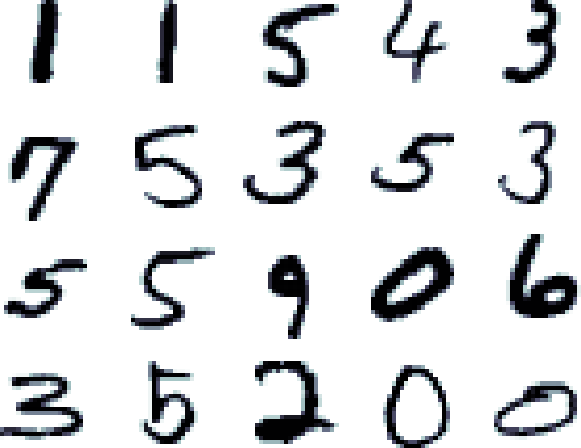
\includegraphics[width = .4\columnwidth]{../fig/mnist_originals.png}
	\caption{Exemple de digits de la base MNIST.}
	\label{MNISTORI}
	\end{figure}
\end{frame}

\subsubsection{Implémentation du RBM}

\begin{frame}{Implémentation du RBM}
	\begin{block}{Gradient analytique}
		\begin{eqnarray}
			\displaystyle \frac{\partial \log \left ( P(x; \theta) \right )}{\partial \theta} =  & - & \displaystyle \sum_{h} P(h|x) \frac{\partial E(x, h; \theta)}{\theta}  \\
			&+& \displaystyle \sum_{x, h} P(x, h) \frac{\partial E(x, h; \theta)}{\partial\theta} 
		\end{eqnarray}
	\end{block}
	Plusieurs techniques de calcul :
	\begin{itemize}
		\item Contrastive divergence (CD)
		\item Persistent Contrastive Divergence
	\end{itemize}
	Utilisation de la bibliothèque scikit-learn qui implémente PCD
\end{frame}

\subsubsection*{Implémentation du MLP}

\begin{frame}{Implémentation du MLP}
	\begin{figure}[ht!]
	\centering
	\begin{tabular}{l|c|c|c|c}
						 &  precision  &  recall & f1-score  & support \\
						0 &      0.90 &     0.96 &     0.93&       174 \\
						1  &     0.67  &    0.58  &    0.62 &      184\\
						2   &    0.86   &   0.87   &   0.86  &     166\\
						3    &   0.75    &  0.74    &  0.75   &    194\\
						4     &  0.86     & 0.85     & 0.86    &   186\\
						5      & 0.75      &0.80      &0.77     &  181\\
						6 &      0.90&      0.94&      0.92      & 207\\
						7  &     0.84 &     0.90  &    0.87&       154\\
						8   &    0.80  &    0.65   &   0.72 &      182\\
						9    &   0.69   &   0.78    &  0.73  &     169\\
	avg / total     &  0.80    &  0.80     & 0.80   &   1797
	\end{tabular}
	\caption{Résultats avec le MLP seul et la petite base MNIST - méthode de classification SVM}
	\end{figure} 
\end{frame}

\subsubsection{Processus complet}

\begin{frame}{Processus complet}
	\begin{algorithm}[H]
	\caption{Entrainement d'un DBN}
	\label{ProcessComplet}
		\begin{algorithmic}
			\State H $\gets$ digits
			\For{currentRBM in RBMs}
					\State Entrainer currentRBM à partir de H
					\If{currentRBM n'est pas le dernier}
						\State Echantillonner une base H
					\EndIf
				\State previousRBM $\gets$ currentRBM
			\EndFor
			
			\State MLP.weights $\gets$ RBMs.weights
			\State Entrainement du MLP à partir de digits
			\State Entrainement de la regression logistique
			
			\State Test à partir d'une base de test
		\end{algorithmic}
	\end{algorithm}
\end{frame}

\subsection{Résultats}

\subsubsection{Petite base + RBM}

\begin{frame}{Résultats du RBM}
	\begin{figure}[ht!]
	\centering
	\begin{tabular}{l|c|c|c|c}
						 &  precision  &  recall & f1-score  & support \\
						0&       0.99   &   0.99    &  0.99   &    174 \\
						1 &      0.92    &  0.95     & 0.93     &  184 \\
						2  &     0.95    &  0.98      &0.97    &   166 \\
						3   &    0.97    &  0.91     & 0.94   &    194 \\
						4    &   0.97    &  0.95    &  0.96  &     186 \\
						5     &  0.93  &    0.93     & 0.93 &      181 \\
						6      & 0.98    &  0.97    &  0.97&       207 \\
						7       &0.95  &    1.00    &  0.97   &    154 \\
						8       &0.90   &   0.88     & 0.89   &    182 \\
						9 &      0.91    &  0.93    &  0.92     &  169 \\
	avg / total  &     0.95    &  0.95    &  0.95    &  1797 \\
	\end{tabular}
	\caption{Résultats avec le RBM seul et la petite base MNIST - méthode de classification régression logistique.}
	\end{figure} 
\end{frame}

\subsubsection{Petite base + DBN}

\begin{frame}{Résultats du DBN sans MLP}
	\begin{figure}[ht!]
	\centering
	\begin{tabular}{l|c|c|c|c}
	& precision   & recall  &f1-score &  support \\
          0&       0.99&      0.98&      0.99&       174\\
          1 &      0.96 &     0.96 &     0.96 &      184\\
          2  &     0.97 &     0.99  &    0.98  &     166\\
          3   &    0.95 &     0.95  &    0.95   &    194\\
          4    &   0.97 &     0.96   &   0.96   &    186\\
          5     &  0.94  &    0.96    &  0.95    &   181\\
          6      & 1.00   &   0.97     & 0.99    &   207\\
          7       &0.94   &   0.99     & 0.97     &  154\\
          8       &0.93   &   0.90     & 0.91     &  182\\
          9       &0.92    &  0.93     & 0.93     &  169\\
avg / total       &0.96     & 0.96     & 0.96     & 1797\\
	\end{tabular}
	\caption{Résultats avec le DBN et la petite base MNIST sans le MLP - méthode de classification régression logistique.}
	\end{figure} 
\end{frame}



\begin{frame}{Résultats du DBN}
	\begin{figure}[ht!]
	\centering
	\begin{tabular}{l|c|c|c|c}
	& precision   & recall  &f1-score &  support \\
          0&       0.99&      0.99&      0.99    &   174 \\
          1 &      0.94 &     0.92 &     0.93    &   184\\
          2  &     0.93  &    0.98  &    0.95       &166\\
          3   &    0.94   &   0.91   &   0.92       &194\\
          4    &   0.97    &  0.91    &  0.94      & 186\\
          5     &  0.94     & 0.91     & 0.92     &  181\\
          6      & 0.98      &0.95      &0.96    &   207\\
          7       &0.93&      0.98&      0.96   &    154\\
          8&       0.86 &     0.92 &     0.89  &     182\\
          9 &      0.89  &    0.93  &    0.91 &      169\\
avg / total  &     0.94   &   0.94   &   0.94&      1797\\
	\end{tabular}
	\caption{Résultats avec le DBN et la petite base MNIST - méthode de classification régression logistique.}
	\end{figure} 
\end{frame}

\subsubsection*{Grande base + DBN}


\begin{frame}{Résultats du DBN}
	\begin{figure}[ht!]
	\centering
	\begin{tabular}{l|c|c|c|c}
           &  precision&    recall&  f1-score&   support\\
        0.0&       0.97 &     0.98 &     0.98 &     1312\\
        1.0 &      0.99  &    0.98  &    0.98  &    1604\\
        2.0  &     0.95   &   0.96   &   0.95   &   1348\\
        3.0   &    0.94    &  0.95    &  0.95    &  1427\\
        4.0    &   0.97     & 0.97     & 0.97     & 1362\\
        5.0      & 0.96      &0.93      &0.94      &1280\\
        6.0     &  0.97&      0.98&      0.97&      1397\\
        7.0       &0.96 &     0.95 &     0.96 &     1461\\
        8.0&       0.94  &    0.96  &    0.95  &    1390\\
        9.0 &      0.94   &   0.94   &   0.94   &   1419\\
avg / total   &    0.96     & 0.96    &  0.96    & 14000
	\end{tabular}
	\caption{Résultats avec le DBN et la grande base MNIST - méthode de classification régression logistique.}
	\end{figure} 
\end{frame}

\begin{frame}{Récapitulatif}
	\begin{figure}[ht!]
	\centering
	\begin{tabular}{|l|c|}
			\hline
			expérience &  f1-score\\
			\hline
			MLP (petite base) & 0.80 \\
			\hline
			RBM (petite base) & 0.95 \\
			\hline
			DBN (petite base) & 0.96 \\
			\hline
			DBN + MLP (petite base) & 0.94 \\
			\hline
			DBN + MLP (grande base) & 0.96 \\
		\hline
	\end{tabular}
	\caption{Récapitulatif des différents résultats.}
	\end{figure} 
\end{frame}